\section{Conclusions}

\begin{frame}
	\frametitle{Conclusions}
		\begin{itemize}
			\item Global error estimation is reduced using Multi-Clustered approach respect to Multi-Filter
			\item Average errors are comparable using all maps
			\item The proposed approach is more robust to false perceptions respect to Multi-Filter approach
			\item The Multi-Clustered Particle Filter algorithm is suitable to be used in dynamic environments due to its
				  characteristics of \emph{reliability} and \emph{robustness}
		\end{itemize}
\end{frame}

\begin{frame}
	\frametitle{Future Works}
	\begin{columns}[T]
		\column{.65\textwidth}
		
		\begin{itemize}
			\item Improving clustering phase
			\item Use systematic noise
			\item Test the architecture in a more decision-driven scenario (like Prey-Predator model)
			\item Evaluate the impact of the algorithm on real-world environment
		\end{itemize}
		
		\column{.35\textwidth}
		\centering
		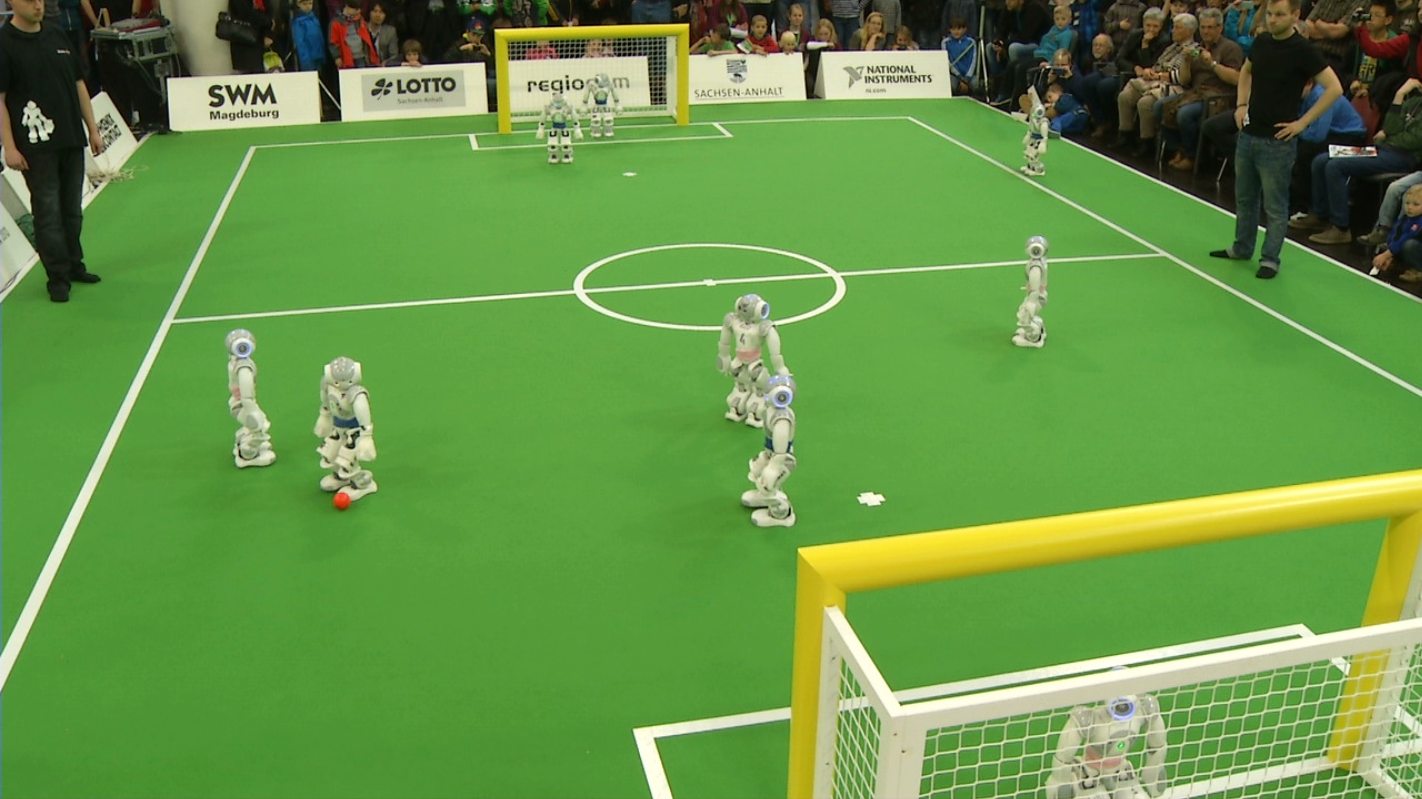
\includegraphics[width=3cm]{Figures/Nao.jpg}
	\end{columns}
\end{frame}

\begin{frame}
	\frametitle{That's all!}
	\begin{center}
		\Large{\textbf{Thank you for your attention}}
	\end{center}
\end{frame}
